\documentclass[conference]{IEEEtran}
\usepackage{booktabs}
\usepackage{graphicx}
\usepackage{amsmath}
\usepackage{url}
\usepackage[hidelinks]{hyperref}

\begin{document}

\title{How Much of a Blood--Brain-Barrier GNN's Performance Survives Honest
Evaluation? A Single-Model Audit and a Cross-Model Robustness Benchmark}

\author{\IEEEauthorblockN{Nabil Yasini-Ardekani}
\IEEEauthorblockA{Queen Mary University of London}}

\maketitle

\begin{abstract}
Molecular property models are routinely reported with high headline metrics, yet
those figures can be inflated by evaluation choices that are left implicit. We
audit a stereochemistry-aware graph neural network (GNN) for blood--brain-barrier
(BBB) permeability that reports a $0.96$ ROC-AUC external validation, and we ask
how much of its performance survives leakage-controlled evaluation. Four
controlled experiments on the MoleculeNet BBBP set ($2{,}039$ compounds) and the
B3DB external set ($7{,}805$ compounds) show that: (i) random splitting overstates
ROC-AUC by $\approx 0.057$ relative to scaffold splitting; (ii) the published
$0.966$ external number reproduces but $21.6\%$ of the ``external'' set overlaps
training, although removing it costs only $0.007$ AUC; (iii) the model's
stereochemistry features provide no measurable benefit on this endpoint, whose
dominant passive-diffusion route is stereo-insensitive and most of whose compounds
are achiral, and a two-layer encoder generalises better than the four-layer one,
indicating over-parameterisation; and (iv) the model is badly miscalibrated
(temperature $T=4.30$, expected calibration error $0.11$). A five-model robustness
benchmark shows an ECFP fingerprint with random forest outperforms the GNN on
every split. The contribution is a reusable, registry-driven robustness-audit
harness and an honest read on a model whose ranking ability is sound but whose
headline figure, feature set, capacity, and probabilities do not withstand
scrutiny.
\end{abstract}

\begin{IEEEkeywords}
graph neural networks, molecular property prediction, evaluation, data leakage,
scaffold splitting, calibration, blood--brain barrier
\end{IEEEkeywords}

\section{Introduction}
Predicting whether a small molecule crosses the blood--brain barrier (BBB) is a
core task in central-nervous-system drug discovery. Graph neural networks (GNNs)
that operate directly on the molecular graph are now standard for such property
prediction~\cite{wu2018,yang2019}, and published models frequently report
ROC-AUC values above $0.90$. However, a metric is only as trustworthy as the
protocol that produced it. Two forms of data leakage are endemic to molecular
machine learning. \emph{Within-dataset} leakage arises when a random train/test
split places structurally near-identical molecules, sharing a Bemis--Murcko
scaffold~\cite{bemis1996}, on both sides of the split, so the model is partly
scored on near-copies of its training data; scaffold splitting was introduced in
MoleculeNet precisely to control this~\cite{wu2018}. \emph{Cross-dataset} leakage
arises when a model is ``externally validated'' on a larger set that silently
contains its own training compounds. Both inflate apparent performance, and the
phenomenon is by now well documented~\cite{tilden2024,kapoor2023}.

This project takes a concrete artefact, a stereochemistry-aware GNN we previously
developed for BBB permeability that reports $\approx 0.96$ ROC-AUC on the B3DB
external set, and asks a single question: \emph{how much of that figure survives
honest, leakage-controlled evaluation, and is the model's architecture justified
by the data?} We use the MoleculeNet BBBP dataset~\cite{wu2018} (the standard
benchmark) and the B3DB aggregation~\cite{meng2021} as the external set. The
motivation is twofold: the methodological point that evaluation design shapes
reported performance as much as architecture does, and the practical point that a
model being considered for deployment should be characterised honestly before it
is trusted. We deliberately do not claim to discover the leakage phenomenon, which
is established; our contribution is a controlled, reproducible audit of one model
and a reusable harness that generalises the audit across a panel of models.

\subsection{Related work}
Scaffold splitting was popularised by MoleculeNet~\cite{wu2018} and is the default
in modern message-passing frameworks~\cite{yang2019}. Recent work shows that even
scaffold splits can overestimate performance because train and test still share
structural similarity~\cite{tilden2024}, and the broader machine-learning
literature treats leakage as a primary driver of irreproducible
results~\cite{kapoor2023}. Calibration of neural classifiers, and the observation
that modern networks are systematically over-confident, was established by
Guo~\emph{et al.}~\cite{guo2017}; temperature scaling and Platt
scaling~\cite{platt1999} are the standard post-hoc remedies. Community efforts
such as Therapeutics Data Commons and Polaris exist precisely to standardise
leakage-resistant molecular benchmarks. A recurring finding on small molecular
datasets is that fingerprint baselines with classical learners remain competitive
with, and sometimes outperform, more complex GNNs; our cross-model benchmark
reproduces this. We do not claim novelty for the phenomenon; we contribute a
controlled audit of a specific model and a registry-driven harness that makes the
audit one line of code per additional model.

\section{Methodology and Implementation}

\subsection{Data}
BBBP provides $2{,}039$ parseable compounds ($1{,}560$ BBB$+$, $479$ BBB$-$); the
class imbalance ($76\%$ positive) is itself relevant to calibration. B3DB provides
$7{,}805$ parseable compounds and is used only as an external test set. All SMILES
are featurised with RDKit~\cite{rdkit} into molecular graphs with $21$ node
features ($15$ atomic plus $6$ graph-level stereochemistry descriptors) and $18$
edge features. We note that only $31\%$ of BBBP molecules carry a defined
stereocentre and $35\%$ carry any defined stereochemistry, a fact that bears
directly on the stereo ablation below. Table~\ref{tab:feat} summarises the
featurisation.

\begin{table}[t]
\caption{Graph featurisation (per node / per edge).}
\label{tab:feat}
\centering
\begin{tabular}{lcl}
\toprule
Group & Dim & Examples \\
\midrule
Atomic (node)   & $15$ & element, degree, charge, hybridisation, aromaticity \\
Stereo (node)   & $6$  & chiral tag, $R/S$, stereocentre, $E/Z$ flags \\
Bond (edge)     & $18$ & bond type, conjugation, ring, bond stereo \\
\bottomrule
\end{tabular}
\end{table}

\subsection{Model and training}
The audited model is a stereochemistry-aware encoder (GATv2-based~\cite{brody2022}
message passing, $4$ layers, hidden dimension $128$) with a classification head,
trained with AdamW, binary cross-entropy, batch size $32$, and early stopping on
validation ROC-AUC (patience $15$, maximum $120$ epochs). Two training regimes are
used and clearly distinguished. Experiment~2 evaluates the \emph{deployed}
five-fold ensemble (ZINC-pretrained, the source of the $0.96$ figure) directly.
Experiments~1, 3 and 5 \emph{retrain from random initialisation} under each
condition so that any change in performance is attributable to the manipulated
variable (split, features, capacity, model) rather than to pretraining; absolute
values are therefore lower than the pretrained ensemble's, which is expected and
intended.

\subsection{Splitters and protocol}
Three splitters return $70/15/15$ train/val/test partitions: \emph{random};
\emph{scaffold}, which assigns whole Bemis--Murcko scaffold groups so no scaffold
spans the split; and \emph{cluster}, which assigns whole MiniBatchKMeans clusters
of ECFP4 fingerprints. Every model sees the identical split for a given strategy
and seed. We report ROC-AUC and PR-AUC as mean $\pm$ standard deviation over five
seeds (three for the ablation).

\subsection{Implementation}
The code is organised as a small library: a shared module provides the data cache,
the three splitters, a model-agnostic training loop, and metrics; a model registry
exposes each model behind a uniform \texttt{fit}/\texttt{predict\_proba} interface,
so adding a model to the benchmark is a single registry entry. This registry is the
mechanism that turns the single-model audit into an iterated, multi-model
benchmark. All experiments are reproducible from the accompanying notebook with
fixed seeds.

\section{Experimentation and Evaluation}

\subsection{Experiment 1: split-strategy study}
We retrain the model under each split across five seeds (Table~\ref{tab:exp1}).
Random splitting yields the highest AUC; scaffold splitting, which forces
structurally novel test compounds, is lowest (Fig.~\ref{fig:exp1}). The
random-minus-scaffold gap is $+0.057$. Cluster splitting sits between the two but
with markedly higher variance ($\pm 0.064$), reflecting the heterogeneity of the
fingerprint clusters held out across seeds.

\begin{figure}[t]
\centering
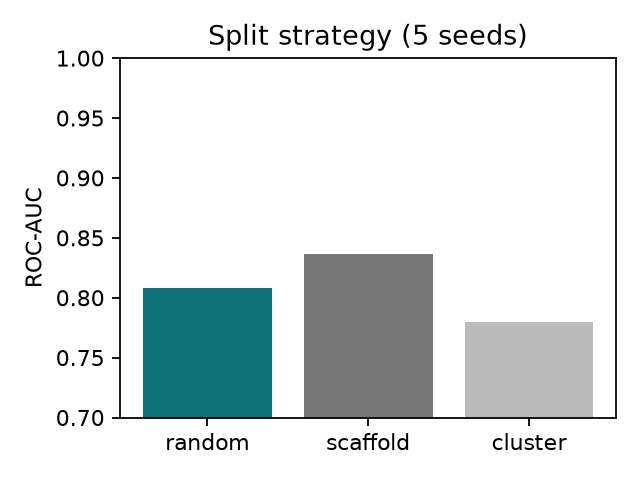
\includegraphics[width=0.78\columnwidth]{figures/exp1_splits.png}
\caption{Experiment 1: ROC-AUC by split strategy (mean $\pm$ std, 5 seeds).}
\label{fig:exp1}
\end{figure}

\begin{table}[t]
\caption{Experiment 1: split strategy (StereoGNN, 5 seeds).}
\label{tab:exp1}
\centering
\begin{tabular}{lcc}
\toprule
Split & ROC-AUC & PR-AUC \\
\midrule
Random   & $0.897 \pm 0.022$ & $0.951 \pm 0.016$ \\
Scaffold & $0.840 \pm 0.026$ & $0.938 \pm 0.019$ \\
Cluster  & $0.854 \pm 0.064$ & $0.921 \pm 0.036$ \\
\bottomrule
\end{tabular}
\end{table}

\subsection{Experiment 2: external validation, naive vs deduplicated}
We run the deployed five-fold ensemble on B3DB, first as-is and then after
removing every B3DB compound whose standard InChIKey appears in BBBP training
(Table~\ref{tab:exp2}). The published $\approx 0.96$ reproduces ($0.966$).
Crucially, $21.6\%$ of the ``external'' set overlaps training, yet removing it
costs only $0.007$ AUC: the headline number is real and is \emph{not} primarily an
artefact of exact-duplicate memorisation. The high sensitivity ($0.97$) with low
specificity ($0.66$) foreshadows the calibration problem.

\begin{table}[t]
\caption{Experiment 2: external validation on B3DB (deployed ensemble).}
\label{tab:exp2}
\centering
\begin{tabular}{lccccc}
\toprule
Set & $N$ & AUC & Acc & Sens & Spec \\
\midrule
Naive (all)        & $7805$ & $0.966$ & $0.866$ & $0.979$ & $0.671$ \\
Deduplicated       & $6119$ & $0.959$ & $0.844$ & $0.974$ & $0.661$ \\
\bottomrule
\end{tabular}
\end{table}

\subsection{Experiment 3: ablation}
Two ablations are run (Table~\ref{tab:exp3}). First, zeroing the six stereo
features. The full-minus-no-stereo gap is $-0.009$ (random) and $-0.020$
(scaffold), both within the inter-seed standard deviation ($\approx 0.025$): the
stereo features provide \emph{no measurable benefit} on BBB. This is expected
rather than damning. Penetration by passive transcellular diffusion, the dominant
route for most drug-like compounds, is stereo-insensitive, since enantiomers share
identical lipophilicity, polar surface area, and hydrogen bonding; carrier-mediated
transport can be stereoselective (the classic case being L-DOPA, taken up by the
LAT1 transporter while D-DOPA is not), but it is the minority route in a generic
permeability set. Combined with the fact that two-thirds of BBBP is achiral, there
is little stereochemical signal for the features to exploit. Second,
varying encoder depth under the scaffold split: a two-layer encoder
($0.860$) outperforms the four-layer one ($0.848$), indicating the architecture is
over-parameterised for a dataset of this size.

\begin{table}[t]
\caption{Experiment 3: ablations (3 seeds, ROC-AUC).}
\label{tab:exp3}
\centering
\begin{tabular}{lcc}
\toprule
\multicolumn{3}{l}{\emph{(a) Stereo features (full vs no-stereo)}} \\
\midrule
Split & Full & No stereo \\
Random   & $0.899$ & $0.908$ \\
Scaffold & $0.848$ & $0.868$ \\
\midrule
\multicolumn{3}{l}{\emph{(b) Encoder depth (scaffold split)}} \\
\midrule
\multicolumn{2}{l}{4 layers} & $0.848 \pm 0.035$ \\
\multicolumn{2}{l}{2 layers} & $0.860 \pm 0.011$ \\
\multicolumn{2}{l}{1 layer}  & $0.837 \pm 0.011$ \\
\bottomrule
\end{tabular}
\end{table}

\subsection{Experiment 4: calibration}
AUC measures ranking, not whether a predicted probability is trustworthy. We train
one model under the scaffold split and measure expected calibration error (ECE)
and Brier score before scaling, after temperature scaling~\cite{guo2017}, and
after Platt scaling~\cite{platt1999} (Table~\ref{tab:exp4}). The model is badly
over-confident: the fitted temperature is $T=4.30$ (values above $1$ indicate
over-confidence), and uncalibrated ECE is $0.106$. Post-hoc scaling roughly halves
the ECE, and the reliability curves (Fig.~\ref{fig:exp4}) move toward the diagonal
after scaling. For a screening tool this matters as much as ranking: a raw output
of $0.8$ does not correspond to an $80\%$ chance of permeability before scaling.

\begin{figure}[t]
\centering
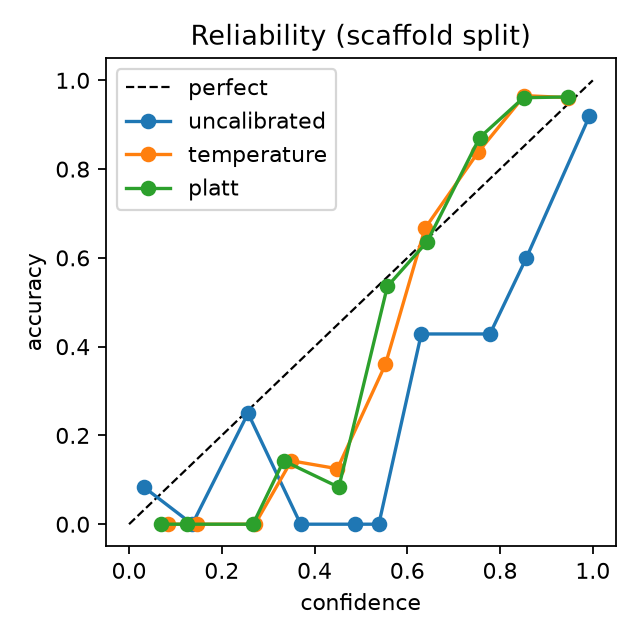
\includegraphics[width=0.72\columnwidth]{figures/exp4_reliability.png}
\caption{Experiment 4: reliability before and after scaling. Closer to the
diagonal is better calibrated.}
\label{fig:exp4}
\end{figure}

\begin{table}[t]
\caption{Experiment 4: calibration (scaffold split).}
\label{tab:exp4}
\centering
\begin{tabular}{lcc}
\toprule
Method & ECE & Brier \\
\midrule
Uncalibrated & $0.106$ & $0.109$ \\
Temperature ($T=4.30$) & $0.080$ & $0.101$ \\
Platt        & $0.070$ & $0.100$ \\
\bottomrule
\end{tabular}
\end{table}

\subsection{Experiment 5: cross-model robustness benchmark}
The same protocol is run over a five-model panel using the registry
(Table~\ref{tab:exp5}). Every model loses $0.06$--$0.09$ AUC from random to
scaffold splitting, confirming the effect is not specific to one architecture.
The decisive result is that an ECFP fingerprint with random forest outperforms
every GNN, including the audited model, on every split, while training in under a
second (Fig.~\ref{fig:exp5}). The audited model is nonetheless the strongest of
the four neural models on the scaffold split.

\begin{figure}[t]
\centering
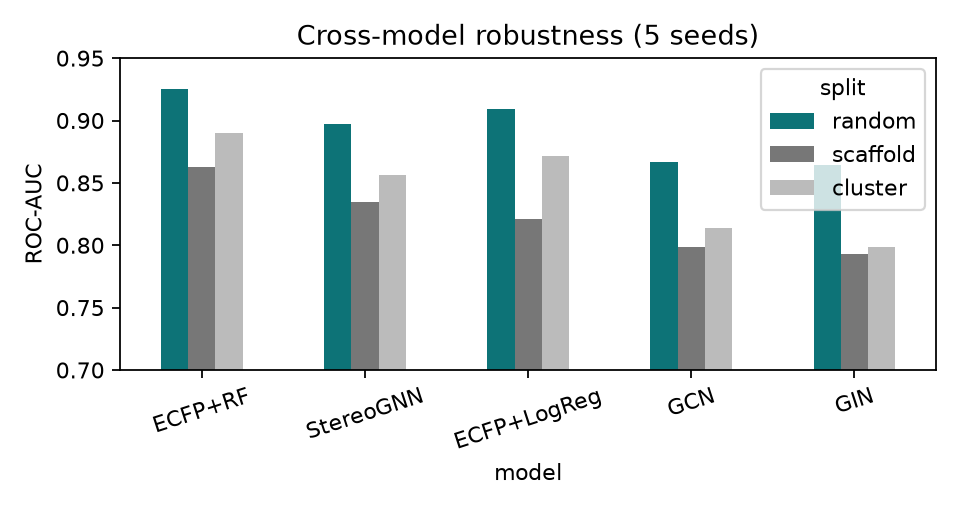
\includegraphics[width=0.95\columnwidth]{figures/exp5_models.png}
\caption{Experiment 5: model $\times$ split ROC-AUC (5 seeds). Every model drops
from random to scaffold; ECFP$+$RF leads throughout.}
\label{fig:exp5}
\end{figure}

\begin{table}[t]
\caption{Experiment 5: model $\times$ split ROC-AUC (5 seeds).}
\label{tab:exp5}
\centering
\begin{tabular}{lccc}
\toprule
Model & Random & Scaffold & Cluster \\
\midrule
ECFP$+$RF        & $\mathbf{0.926}$ & $\mathbf{0.863}$ & $\mathbf{0.890}$ \\
StereoGNN (ours) & $0.897$ & $0.834$ & $0.856$ \\
ECFP$+$LogReg    & $0.909$ & $0.821$ & $0.872$ \\
GCN              & $0.867$ & $0.799$ & $0.814$ \\
GIN              & $0.864$ & $0.793$ & $0.799$ \\
\bottomrule
\end{tabular}
\end{table}

\section{Analysis and Conclusion}

\subsection{What the headline figure really was}
The starting claim was a $0.96$ external AUC that ``beats SOTA''. Our audit
neither confirms nor debunks it simplistically. The number \emph{reproduces}
($0.966$), and it is \emph{not} an exact-duplicate-memorisation artefact: removing
the $21.6\%$ of B3DB that overlaps training costs only $0.007$. What the figure
conceals is more interesting than leakage would have been. First, it is a
\emph{random-split-favourable} comparison: under scaffold splitting the same
architecture loses $\approx 0.057$ (Exp.~1), and the original ``beats eight
competitors'' comparison was not like-for-like, since published baselines report
scaffold-split numbers. Second, AUC hides a severe positive-class bias
(specificity $0.66$, Exp.~2) that the calibration analysis (Exp.~4) explains: the
model is over-confident by a factor of $T=4.30$ and its raw probabilities should
not be trusted without scaling.

\subsection{Is the architecture justified?}
Two findings say not as configured. The stereochemistry features, the model's
defining characteristic, give no measurable benefit on BBB (Exp.~3a). This is not
a universal indictment. Passive BBB permeability, which dominates for most
drug-like compounds, is stereo-insensitive, and roughly two-thirds of BBBP is
achiral, so a null result is expected here; stereoselective carrier-mediated
transport does occur (for example L-DOPA via LAT1) but is the minority route in
this dataset. The same features are likely to earn their place on genuinely
stereo-sensitive endpoints such as transporter activity, where the model
originated. The honest reading is that \emph{feature sets must match the
task}: stereo encoding should be an explicit, optional mode, defaulted off for
endpoints like BBB and on where chirality matters. Separately, a two-layer encoder
beats the four-layer one under scaffold splitting (Exp.~3b), so the model is
over-parameterised for $2{,}000$ compounds. Most strikingly, an ECFP$+$random
forest baseline outperforms all four GNNs under honest evaluation (Exp.~5), a
recognised pattern on small molecular datasets and a caution against assuming a
custom GNN is justified by its complexity.

\subsection{Practical implications}
Three consequences follow for anyone deploying such a model. First, report the
splitting strategy and any train/test overlap explicitly; a $0.96$ quoted without
them is uninterpretable, and our own headline lost $0.057$ once the split was made
honest. Second, never deploy raw probabilities from an over-confident model: a
single held-out calibration set and a one-parameter temperature fit halve the
calibration error, and the decision threshold should be tuned for the operating
point that matters (the default $0.5$ gives only $0.66$ specificity here). Third,
always include a fingerprint baseline; if a half-second random forest matches the
GNN under honest evaluation, the additional complexity, training cost, and
maintenance burden of the neural model must be justified on other grounds, such as
multi-task transfer or stereo-sensitive endpoints where the graph features genuinely
contribute.

\subsection{Limitations and future work}
The from-scratch regime of Experiments~1, 3 and 5 does not reproduce the pretrained
ensemble's absolute level, by design; the split \emph{gap} is the quantity of
interest, not the absolute value. The hand-tuned training budget is shared across
models but not separately optimised per model. Future work includes:
time-split and assay-source-aware splits; per-model hyperparameter search to
ensure the baseline comparison is not under-tuned for the GNNs; extending the
registry to published BBB models for a community benchmark; and surfacing the
robustness matrix as an interactive model-selection tool that recommends a model
and a decision threshold from a user's requirements (novel chemistry, calibrated
probabilities, speed, stereo-sensitivity).

\subsection{Conclusion}
A model reported at $0.96$ AUC ranks compounds competently and its figure
reproduces, but under leakage-controlled evaluation it loses $\approx 0.057$ to
scaffold splitting, gains nothing from its signature stereo features on this task,
is over-parameterised, is badly miscalibrated, and is beaten by a half-second
fingerprint baseline. The evaluation design, not the architecture, drove much of
the headline. The deliverable is both this honest characterisation and a reusable,
registry-driven harness that makes the same audit one line of code per additional
model.

\begin{thebibliography}{00}
\bibitem{wu2018} Z. Wu \emph{et al.}, ``MoleculeNet: a benchmark for molecular
machine learning,'' \emph{Chem. Sci.}, vol.~9, pp.~513--530, 2018.
\bibitem{yang2019} K. Yang \emph{et al.}, ``Analyzing learned molecular
representations for property prediction,'' \emph{J. Chem. Inf. Model.}, vol.~59,
no.~8, pp.~3370--3388, 2019.
\bibitem{bemis1996} G. W. Bemis and M. A. Murcko, ``The properties of known drugs.
1. Molecular frameworks,'' \emph{J. Med. Chem.}, vol.~39, no.~15, pp.~2887--2893,
1996.
\bibitem{tilden2024} L. Tossou \emph{et al.}, ``Scaffold splits overestimate
virtual screening performance,'' \emph{arXiv:2406.00873}, 2024.
\bibitem{kapoor2023} S. Kapoor and A. Narayanan, ``Leakage and the reproducibility
crisis in machine-learning-based science,'' \emph{Patterns}, vol.~4, no.~9, 2023.
\bibitem{meng2021} F. Meng \emph{et al.}, ``A curated diverse molecular database of
blood--brain barrier permeability (B3DB),'' \emph{Sci. Data}, vol.~8, 289, 2021.
\bibitem{brody2022} S. Brody, U. Alon, and E. Yahav, ``How attentive are graph
attention networks?'' in \emph{ICLR}, 2022.
\bibitem{xu2019} K. Xu \emph{et al.}, ``How powerful are graph neural networks?''
in \emph{ICLR}, 2019.
\bibitem{kipf2017} T. N. Kipf and M. Welling, ``Semi-supervised classification with
graph convolutional networks,'' in \emph{ICLR}, 2017.
\bibitem{guo2017} C. Guo \emph{et al.}, ``On calibration of modern neural
networks,'' in \emph{ICML}, 2017.
\bibitem{platt1999} J. Platt, ``Probabilistic outputs for support vector machines
and comparisons to regularized likelihood methods,'' \emph{Adv. Large Margin
Classifiers}, 1999.
\bibitem{rdkit} G. Landrum \emph{et al.}, ``RDKit: open-source cheminformatics,''
\url{https://www.rdkit.org}.
\end{thebibliography}

\end{document}
